\section{One-Dimensional Systems}
\noindent\rule[\linienAbstand]{\linewidth}{\linienDickeDick}

\subsection{Fixed Points in Continuous Dynamical Systems}
\noindent\rule[\linienAbstand]{\linewidth}{\linienDicke}
A \emph{fixed point} of the a continuous dynamical system is an $x^*$ with the property
\begin{equation}
  \dot{x} = f(x^*) = 0
\end{equation}
If $x^*$ is a fixed point, then $x(t) = x^*$ is a constant solution of the system.\\

For the solution $x(t)$ of a one-dimensional system there are the following possibilites:
\begin{itemize}
  \item The solution is a fixed point
  \item The solution grows monotonically, i.e. $\dot{x}(t) > 0$
  \item The solution decays monotonically, i.e. $\dot{x}(t) < 0$
\end{itemize}

Example: We consider the ODE of limited growth
\begin{equation}
  \dot{N} = rN\left(1-\frac{N}{K}\right)
\end{equation}
If $K = 1$, $\dot{N}$ is $0$ if $N = 0$ and $N = 1$ i.e. the fixed points for this equation are $x_1 = 0$ and $x_2 = 1$ (or $x_2 = K$). These fixed points are also visible in the following figure.

\begin{figure}[H]
  \centering
  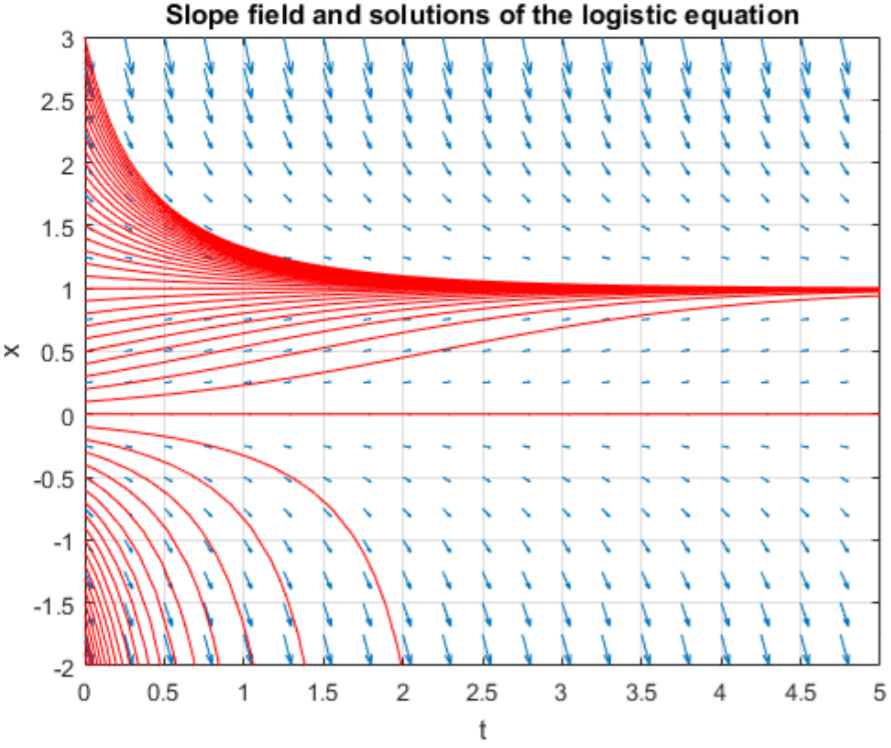
\includegraphics[width=.7\linewidth]{Pics/4.2.png}
\end{figure}

\subsection{Continuous Linear stability analysis}
\noindent\rule[\linienAbstand]{\linewidth}{\linienDicke}
Let $x^*$ be a fixed point of the continuous dynamical system $\dot{x} = f(x)$. The fixed point $x^*$ is
\begin{itemize}
  \item stable if $f'(x^*) < 0$,
  \item unstable, if $f'(x^*) > 0$,
  \item stable or unstable, if $f'(x^*) = 0$
\end{itemize}

Example (continuation): the derivative of the logistic equation above $\left(f(x) = rx\left(1-\frac{x}{K}\right)\right)$ is
\begin{equation}
  f'(x) = r\left(1-\frac{2x}{K}\right)
\end{equation}
Hence
\begin{equation}
  \begin{split}
    f'(x_1) =& f'(0) = r > 0\\
    f'(x_2) =& f'(K) = -r < 0
  \end{split}
\end{equation}
Hence $x_1 = 0$ is an unstable fixed point, and $x_2 = K$ is a stable fixed point, which is also visible in the figure above.

\subsection{Fixed points in Discrete Dynamical Systems}
\noindent\rule[\linienAbstand]{\linewidth}{\linienDicke}
A \emph{fixed point} of the discrete dynamical system $x_{n+1} = f(x_n)$ is a $x^*$ with the property
\begin{equation}
  x^* = f(x^*)
\end{equation}
If $x^*$ is a fixed point of $x_{n+1} = f(x_n)$, then $x_n = x^*$ is a constant solution of that system.\\

Example: We want to find the fixpoint of the discrete dynamical system
\begin{equation}
  x_{n+1} = \textup{cos}(x_n)
\end{equation}
Using the formula above:
\begin{equation}
  x^* = \textup{cos}(x^*) \:\;\; \Rightarrow \;\;\; x^* \approx 0.739
\end{equation}

\subsection{Discrete Linear stability analysis}
\noindent\rule[\linienAbstand]{\linewidth}{\linienDicke}
Let $x^*$ be a fixed point of the discrete dynamical system $x_{n+1} = f(x_n)$. The fixed point $x^*$ is
\begin{itemize}
  \item stable, if $|f'(x^*)| < 1$,
  \item unstable, if $|f'(x^*)| > 1$,
  \item stable or unstable, if  $|f'(x^*)| = 1$
\end{itemize}

\begin{equation}
  \eta_{n+1} = \eta_n \cdot f'(x^*) \;\;\; \Rightarrow \;\;\;
  \eta_n = \eta_0 \cdot \left(f'(x^*)\right)^n
\end{equation}

Example: (continuation): We want to analyse the fixpoint $x^* \approx 0.739$ of the example above.
\begin{equation}
  |f'(x^*)| = |\textup{sin}(x^*)| \approx |-0.674| < 1
\end{equation}
Hence $x^*$ is a stable fixed point of the system.

\subsection{Bifurcations in Continous Systems}
\noindent\rule[\linienAbstand]{\linewidth}{\linienDicke}

\textbf{Fundamentals}\\
A qualitative change of the dynamics of a dynamical system
\begin{equation}
  \dot{x} = f(x, r) \;\;\; \text{or} \;\;\; x_{n+1} = f(x_n, r)
\end{equation}
depending on a parameter $r$ is a bifurcation of the system\\

\textbf{Standard Bifurcations in descrete systems}\\
\textbf{Saddle-node Bifurcation}\\
The saddle-node bifurcation is a bifurcation in which fixed points are created or destroyed by the variation of a system parameter.\\
Example: Dynamical system, depending on the parameter $r$
\begin{equation}
  \dot{x} = r + x^2
\end{equation}
Fixed points:
\begin{equation}
  \begin{split}
    r& < 0: x^*_{1, 2} = \pm\sqrt{-r}\\
    r& = 0: x^* = 0\\
    r& > 0: \text{none}
  \end{split}
\end{equation}
Stability of the fixed points for $r<0$:
\begin{equation}
  f(x) = r + x^2, \;\;\; f'(x) = 2x
\end{equation}
hence
\begin{equation}
  \begin{split}
    x^*_1 &= \sqrt{-r} > 0: f'(x^*_1) > 0, unstable\\
    x^*_2 &= -\sqrt{-r} < 0: f'(x^*_2) < 0, stable\\
  \end{split}
\end{equation}
\begin{figure}[H]
  \centering
  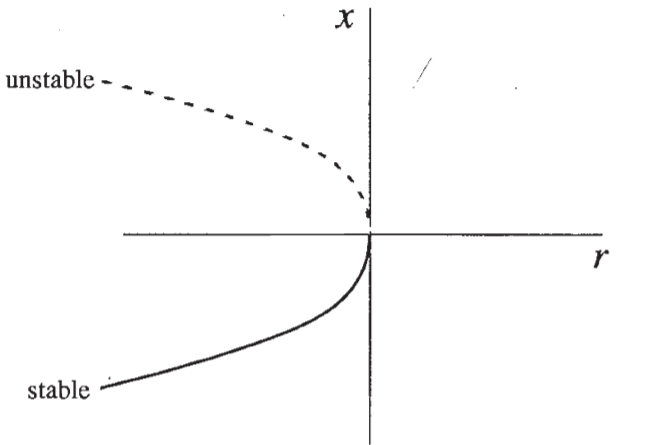
\includegraphics[width=.5\linewidth]{Pics/9.1.png}
\end{figure}

\textbf{Pitchfork Bifurcation}\\
The pitchfork bifurcation is a bifurcation in which a fixed point changes its stability and two new fixed points are created.\\
\begin{table}[H]
  \setlength{\tabcolsep}{0.2em}
  \footnotesize
  \begin{tabular}{p{\linewidth / 2 - 0.5em}@{\hskip 1em}p{\linewidth / 2 - 0.5em}}
    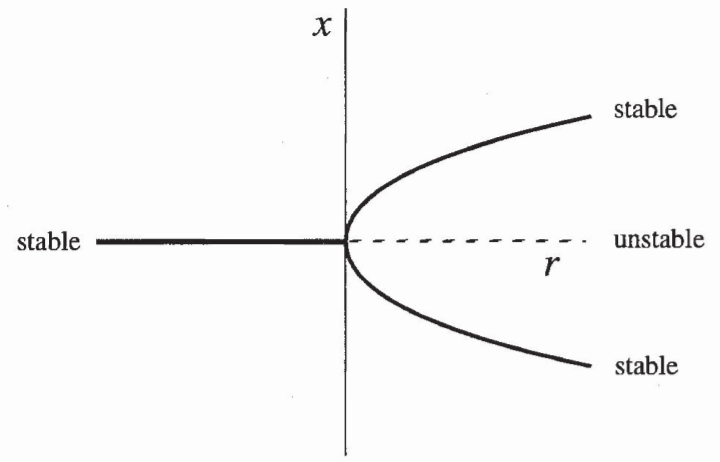
\includegraphics[width=\linewidth]{Pics/9.2.png} & 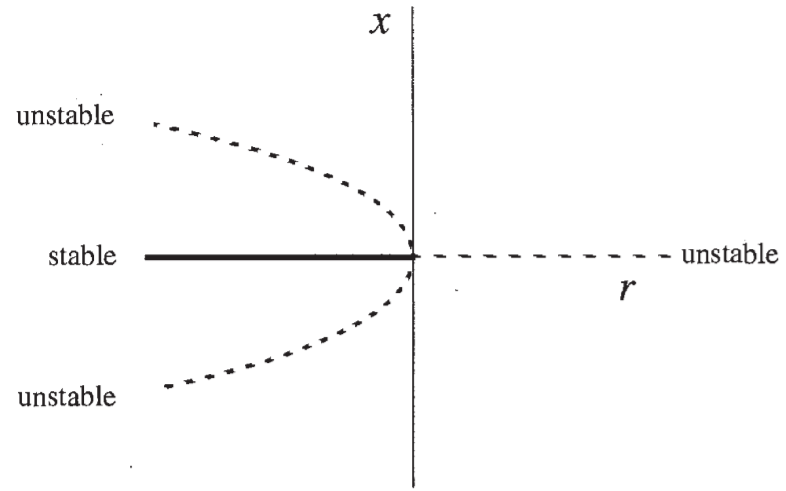
\includegraphics[width=\linewidth]{Pics/9.3.png}\\
    Supercritical & Subcritical
  \end{tabular}
\end{table}
Supercritical: Additional fixed points only for parameter values greater (“super”) than the bifurcation point.\\
Subcritical: Additional fixed points only for parameter values smaller (“sub”) than the bifurcation point.\\

\textbf{Transcritical Bifurcation}\\
A transcritical bifurcation is a bifurcation in which the stability of two fixed points is interchanged.
\begin{figure}[H]
  \centering
  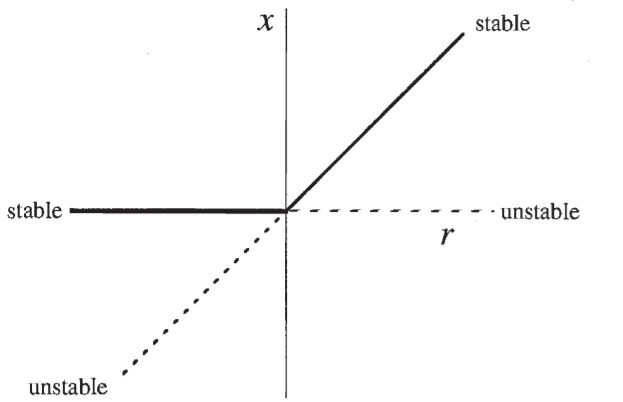
\includegraphics[width=.5\linewidth]{Pics/9.4.png}
\end{figure}

\subsection{Bifurcations in Discrete Systems}
\noindent\rule[\linienAbstand]{\linewidth}{\linienDicke}
The bifurcations which we introduced in continuous systems can also occur in discrete systems.\\
Discrete systems can (or do allways?) show a chaotic behaviour in the parameter space:

\begin{figure}[H]
  \centering
  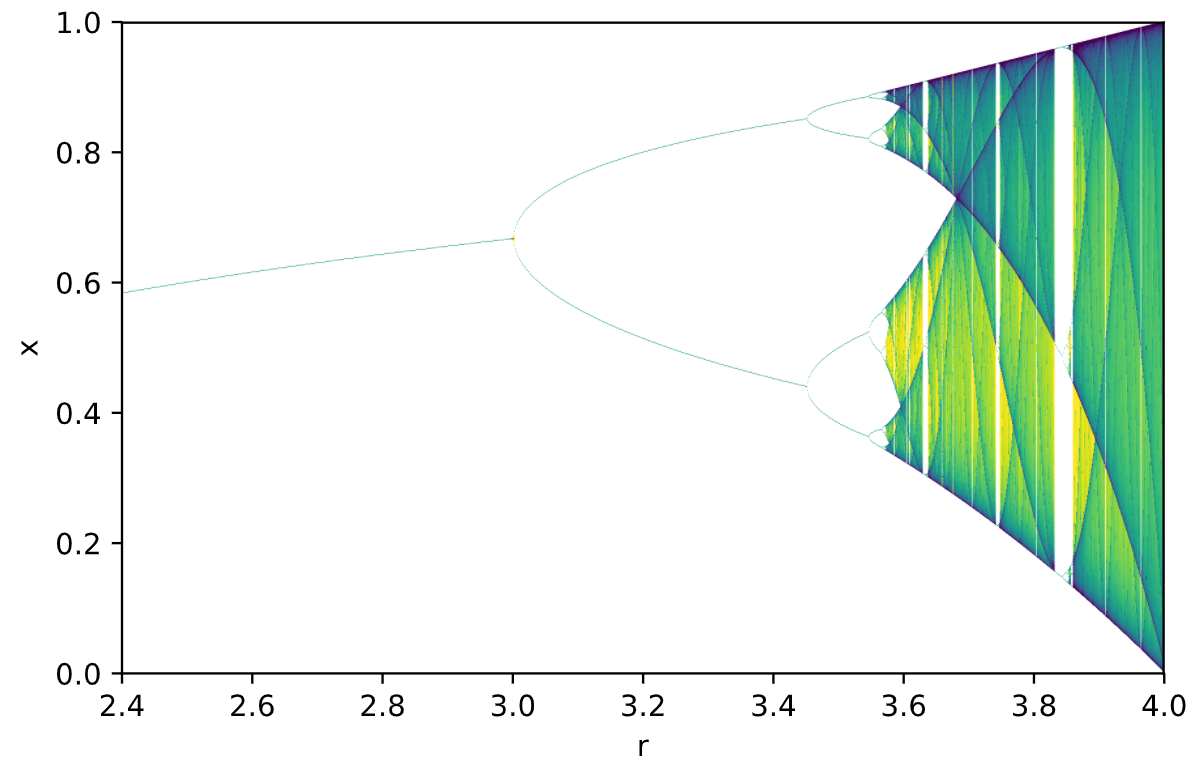
\includegraphics[width=.9\linewidth]{Pics/9.5.png}
\end{figure}

Example: Consider the discrete dynamical system depending on the parameters $\mu \geq 0, \varepsilon \geq 0$ (Adler system)
\begin{equation}
  x_{x+1} = x_n + \mu + \varepsilon \; \textup{sin}(x_n) \;\;\; (\mu \geq 0, \varepsilon \geq 0)
\end{equation}
Fixed points $x^*$ are solutions of the equation $\mu + \varepsilon \; \textup{sin}(x) = 0$, hence
\begin{equation}
  x^*_{1, k} = -\textup{arcsin}\left(\frac{\mu}{\varepsilon}\right) + k \cdot 2\pi, \;\;
  x^*_{2, k} = (2k + 1)\pi + \textup{arcsin}\left(\frac{\mu}{\varepsilon}\right)
\end{equation}
The fixed points only exist in the case $\mu \leq \varepsilon$\\
For $\mu = 1$, the fixed points only exist in the case $\varepsilon \geq 1$. We have $f(x) = x + \mu + \varepsilon \; \textup{sin}(x)$, hence $f'(x) = 1 + \varepsilon \; \textup{cos}(x)$. It follows that for $\mu = 1$
\begin{equation}
  \begin{split}
    f'(x^*_{1, k}) =& 1 + \varepsilon \; \textup{cos}\left(-\textup{arcsin}\left(\frac{1}{\varepsilon}\right)\right)\\
    =& 1 + \varepsilon \sqrt{1 - \frac{1}{\varepsilon^2}}\\
    =& 1 + \sqrt{\varepsilon^2 - 1} \geq 1
  \end{split}
\end{equation}
Hence the fixed points $x^*_{1, k}$ are unstable.
\begin{equation}
  \begin{split}
    f'(x^*_{2, k}) =& 1 + \varepsilon \; \textup{cos}\left(\pi + \textup{arcsin}\left(\frac{1}{\varepsilon}\right)\right)\\
    =& 1 - \varepsilon \; \textup{cos}\left(\textup{arcsin}\left(\frac{1}{\varepsilon}\right)\right)\\
    =& 1 - \varepsilon \sqrt{1 - \frac{1}{\varepsilon^2}}\\
    =& 1 + \sqrt{\varepsilon^2 - 1}
  \end{split}
\end{equation}
For the stability of $x^*_{2, k}$ it is necessary that $|1 - \sqrt{\varepsilon^2-1} < 1$ holds. This is true if and only if $0 < \sqrt{\varepsilon^2 - 1} < 2$, hence in the case $1 < \varepsilon^2 < $5 resp. $1 < \varepsilon < \sqrt{5}$. The fixed points $x^*_{2, k}$ are thus stable in the case $1<\varepsilon<\sqrt{5}$.
